\documentclass[border=2mm]{standalone}
\usepackage    {tikz}
\usetikzlibrary{3d}
\usetikzlibrary{calc}

\begin{document}
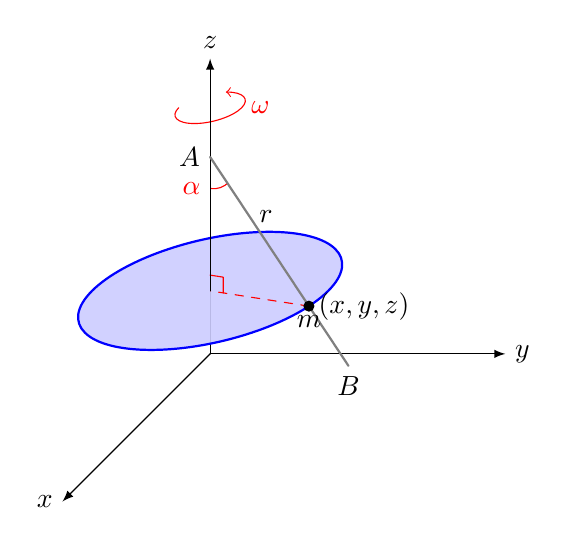
\begin{tikzpicture}[line cap=round,line join=round,
  x={(-0.5cm,-0.5cm)},y={(1cm,0cm)},z={(0cm,1cm)},        % cavalier axes 
%  x={(-0.86cm,-0.5cm)},y={(0.86cm,-0.5cm)},z={(0cm,1cm)}  % isometric axes
  ]
  \def\ha{2.5}  % A height
  \def\hc{0.8}  % circle height
  \def\rc{1.5}  % circle radius
  \def\am{75}   % angle for m and B
  \coordinate (O) at (0,0,0);
  \coordinate (A) at (0,0,\ha);
  \coordinate (C) at (0,0,\hc); % circle center
  \coordinate (m) at ($(C)+(\am:\rc)$);
  \coordinate (B) at ($(A)!1.4!(m)$);
  % AXES
  \draw[-latex] (O) -- (1.5*\ha,0,0) node [left]  {$x$};
  \draw[-latex] (O) -- (0,1.5*\ha,0) node [right] {$y$};
  \draw         (O) -- (C);
  % circle (filled and not)
  \draw[thick,blue,canvas is xy plane at z=\hc,fill=blue!20,fill opacity=0.9] (0,0) circle (\rc);
%  \draw[thick,blue,canvas is xy plane at z=\hc] (0,0) circle (\rc);
  % angles
  \begin{scope}[rotate around z=\am, canvas is xz plane at y=0]
    \draw[red]    ($(C)+(0.2,0)$)  |- ($(C)+(0,0.2)$);
    \node[red] at ($(A)+(0,-0.4)$) [left] {$\alpha$};
    \clip (O) -- (A) -- (B) -- cycle;
    \draw[red]   (A) circle (0.4);
    \draw[red,dashed] (m) -- (C);
  \end{scope}
  \begin{scope}[canvas is xy plane at z=1.25*\ha]
    \draw[red,canvas is xy plane at z=1.25*\ha,->] (0,-0.4) arc (-90:180:0.4);
    \node[red] at (0,0.4) [right] {$\omega$};
  \end{scope}
  % line AB and points
  \draw[-latex] (C) -- (0,0,1.5*\ha) node [above] {$z$}; % top part of z axis
  \draw[thick,gray] (A) node [black,left] {$A$} -- (B) node [black,below] {$B$};
  \fill (m) circle (2pt) node [right] {$(x,y,z)$};
  \node at (m) [below] {$m$};
  \node at ($(A)!0.4!(m)$) [right] {$r$};
\end{tikzpicture}
\end{document}